%%%%%%%%%%%%%%%%%%%%%%%%%%%%%%%%%%%%%%%%%
% Dreuw & Deselaer's Poster
% LaTeX Template
% Version 1.0 (11/04/13)
%
% Created by:
% Philippe Dreuw and Thomas Deselaers
% http://www-i6.informatik.rwth-aachen.de/~dreuw/latexbeamerposter.php
%
% This template has been downloaded from:
% http://www.LaTeXTemplates.com
%
% License:
% CC BY-NC-SA 3.0 (http://creativecommons.org/licenses/by-nc-sa/3.0/)
%
%%%%%%%%%%%%%%%%%%%%%%%%%%%%%%%%%%%%%%%%%

%----------------------------------------------------------------------------------------
%	PACKAGES AND OTHER DOCUMENT CONFIGURATIONS
%----------------------------------------------------------------------------------------

\documentclass[final,hyperref={pdfpagelabels=false}]{beamer}

\usepackage[orientation=portrait,size=a0,scale=1.4]{beamerposter} % Use the beamerposter package for laying out the poster with a portrait orientation and an a0 paper size

\usetheme{I6pd2} % Use the I6pd2 theme supplied with this template

\usepackage[english]{babel} % English language/hyphenation

\usepackage{amsmath,amsthm,amssymb,latexsym} % For including math equations, theorems, symbols, etc

%\usepackage{times}\usefonttheme{professionalfonts}  % Uncomment to use Times as the main font
%\usefonttheme[onlymath]{serif} % Uncomment to use a Serif font within math environments

\boldmath % Use bold for everything within the math environment

\usepackage{booktabs} % Top and bottom rules for tables

\graphicspath{{figures/}} % Location of the graphics files
\usepackage{tikz}
\usecaptiontemplate{\small\structure{\insertcaptionname~\insertcaptionnumber: }\insertcaption} % A fix for figure numbering

%----------------------------------------------------------------------------------------
%	TITLE SECTION 
%----------------------------------------------------------------------------------------

\title{\huge ESS-CAR/NW} % Poster title

\author{Jonas Ekman, Leon Fernandez, Yini Gao, Fredrik Hyyrynen, Jacob Kimblad and  Yifan Ruan} % Author(s)

\institute{ MF2063 Embedded Systems Design Project} % Institution(s)

%----------------------------------------------------------------------------------------
%	FOOTER TEXT
%----------------------------------------------------------------------------------------

\newcommand{\leftfoot}{ESS-CAR/NW} % Left footer text

\newcommand{\rightfoot}{MF2063} % Right footer text

%----------------------------------------------------------------------------------------

\begin{document}
\addtobeamertemplate{headline}{} 
{\begin{tikzpicture}[remember picture, overlay]
     \node [anchor=north east, inner sep=0.5cm]  at (current page.north east)
     {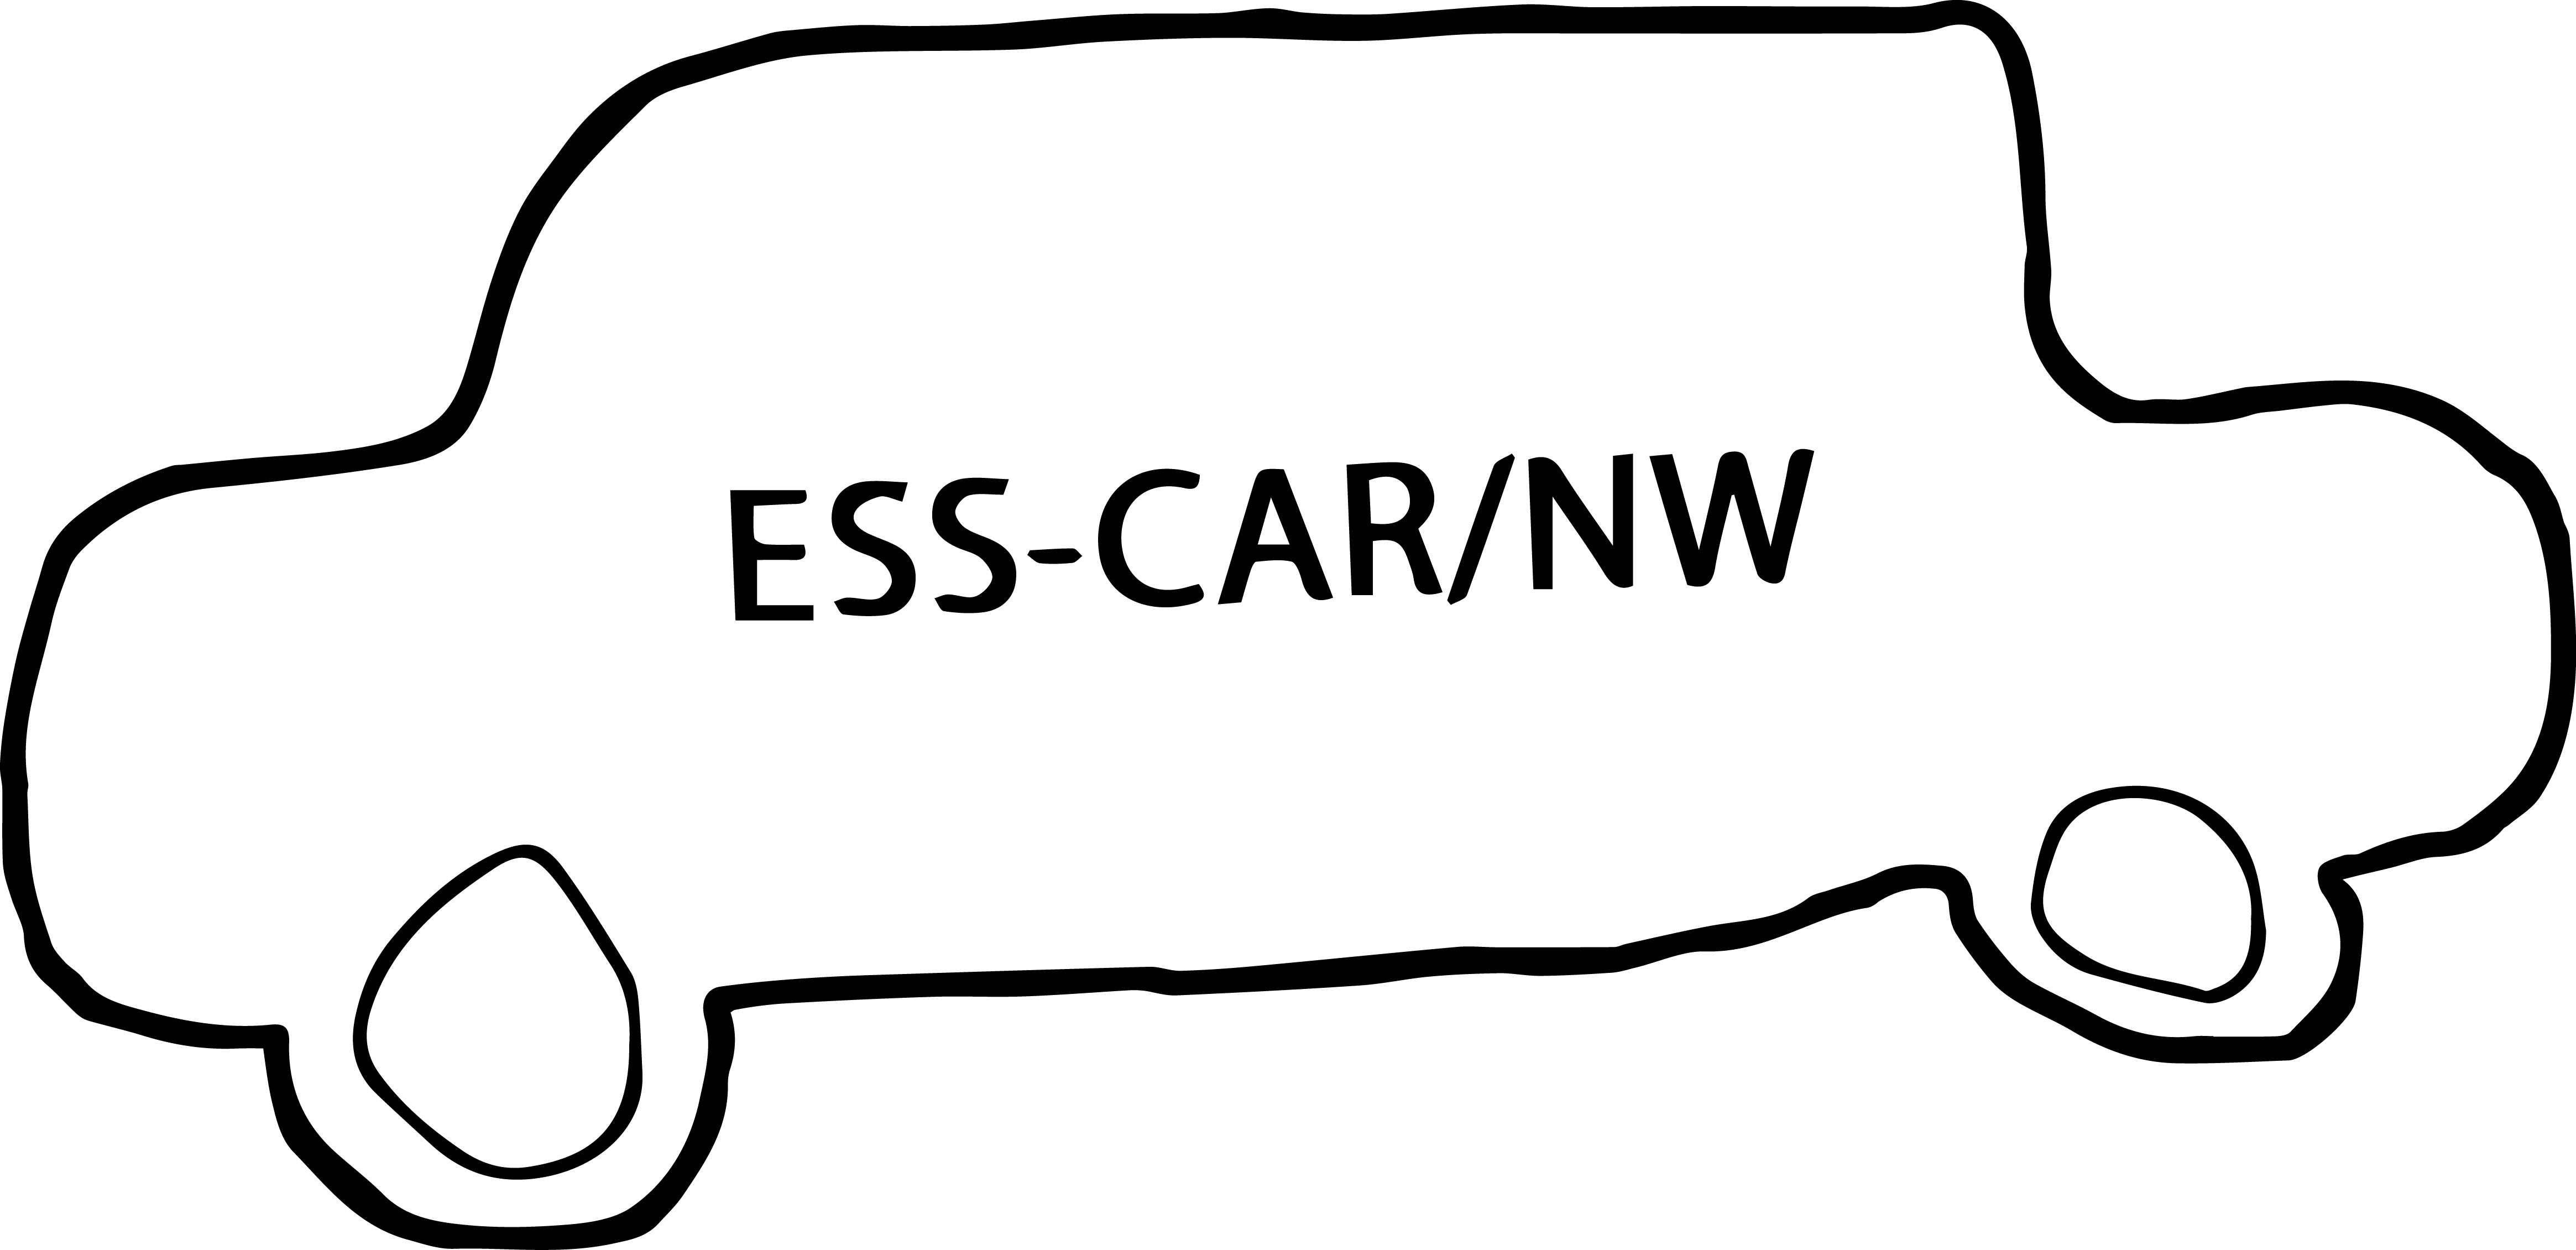
\includegraphics{LogoFun.png}};
     \hspace{4cm}
  \end{tikzpicture}}
\addtobeamertemplate{block end}{}{\vspace*{2ex}} % White space under blocks

\begin{frame}[t] % The whole poster is enclosed in one beamer frame

\begin{columns}[t] % The whole poster consists of two major columns, each of which can be subdivided further with another \begin{columns} block - the [t] argument aligns each column's content to the top

\begin{column}{.02\textwidth}\end{column} % Empty spacer column

\begin{column}{.465\textwidth} % The first column


%----------------------------------------------------------------------------------------
%	INTRODUCTION
%----------------------------------------------------------------------------------------
            
\begin{block}{Introduction}

\begin{itemize}
\item This project is about the implementation of an autonomous car that utilizes a software-defined network (SDN) for communication between a set of nodes. SDN is a new type of technology that moves the control part in the switches to a separate controlling node. Communication over the network is done via the VSOME/IP middleware. It is an application middleware that is designed for the car industry and is compatible with AUTOSAR. On the car are different types of sensors used to monitor the car performance and its surrounding. The sensor and actuator communication is done via controllers and the SDN network. 
\end{itemize}

\end{block}
%
%\begin{block}{Requerments}
%    This is the design requirement for the ESS-CAR
%    \begin{itemize}
%        \item Design and evaluate the software- and system-architecture %for the model car platform. The
%        architecture shall integrate (and potentially adapt) already %existing functionality to achieve a robust and
%        predictable system design.
%
%        \item Setup the physical platform to use different sensors and %actuators (ultrasonic sensor, IR sensor,
%        accelerometer, servo, motor, etc.). The peripherals shall be %controlled with dedicated microcontrollers
%        (Arduino). SPI bus is used to communicate between Arduinos and %Beagle Bone ECUs. Software on the
%        Beagle Bone ECUs shall provide the respective services to t
%        he system using SOME/IP.
%
%        \item Setup the camera module for the Raspberry Pi ECU. This %requires the physical setup (mounting the
%        camera and designing the hardware to do so) but also a software %service that will make the camera
%        data (e.g. traffic sign detection through AI algorithm) %available to other software components over
%        the SOME/IP middleware. This software service shall be %configurable to switch between different
%        quality modes that will affect the produced network load.
%        4) Setup a display that will be mounted on the car. The display %service shall be located on a different
%        ECU than the camera node. The basic functionality is the display %of the video stream that is provided
%        by the camera.
%
%        \item Identify some typical fault models, design and implement %the fault injectors that inject the faults
%        on the network nodes and switches.
%
%        \item Monitor traffic on the ECUs to detect fault conditions and %trigger reconfiguration.
%        \item Develop coordinated boot and shutdown sequences to %efficiently use the model car.
%        \item Write a project report documenting the details of %functional blocks and services, as well as basic
%        system evaluation results.
%
%
%
%        
%    \end{itemize}
%
%    For the ESS-NW is the following the requirements
%    \begin{itemize}
%        \item Build the model car(s) with Turnigy SCT 2WD 1/10 Brushless %Short Course Truck
%        (KIT) upgraded version.
%
%        \item Set up the physical embedded system platform consisting of %BeagelBoneBlack
%        nodes and Zodiac FX SDN-Switches, plus one Raspberry Pi as
%        SDN-Controller and Arduino To interface with sensors and %actuators.
%
%        \item Investigate available implementations of SDN-Controller %and select one that best
%        meets the project requirements.
%
%        \item Design and implement a basic SDN-Controller application on %one of the ECUs.
%        
%        \item Extend the SDN-Controller to manually assign network flows %to preconfigured
%        routes with defined monitoring points on the switches.
%
%        \item Extend the SDN-Controller in a way that the network %resources are reassigned
%        during runtime if message behaviour changes. This requires %monitoring of
%        messages on the switches and reconfiguration of the network at %runtime.
%
%        \item Write a project report documenting the details of %functional blocks and services, as
%        well as basic system evaluation results.
%    \end{itemize}
%    
%\end{block}
%
%%----------------------------------------------------------------------------------------
%	NETWORK
%----------------------------------------------------------------------------------------

\begin{block}{Network}
    \begin{itemize}
        \item Software defined network (SDN) is a type of network configuration that moves the intelligence from the switches to a controller unit. This makes the network smarter and more dynamic. It can sort packages depending on their priorities and traffic load to different paths, to enable faster computing and a better distribution of the network load. It is self-configured when a link goes down or a new link opens up. The SDN is implemented using the OpenFlow protocol for controlling the switches. 
        
        \item Three SDN enabled switches from Zodiac FX is used in this project and the network is configured according to the topology in figure \ref{pic:network}. The controller is a Raspberry Pi model 3 that uses the RYU SDN framework to control the switches and to gather network information. 
        
        \item Information is sent between the nodes using a middleware application called VSOME/IP which is designed for automotive products e.g. cars and is compatible with AUTOSAR. 
        
        \item Arduinos are used on the edge of the network, to control sensors and actuators. The data is then passed via an SPI interface to a BeagleBone Black that for processing and transporation out in the SDN.  
    \end{itemize}

\end{block}

\begin{block}{Network Figure}
    \begin{figure}
        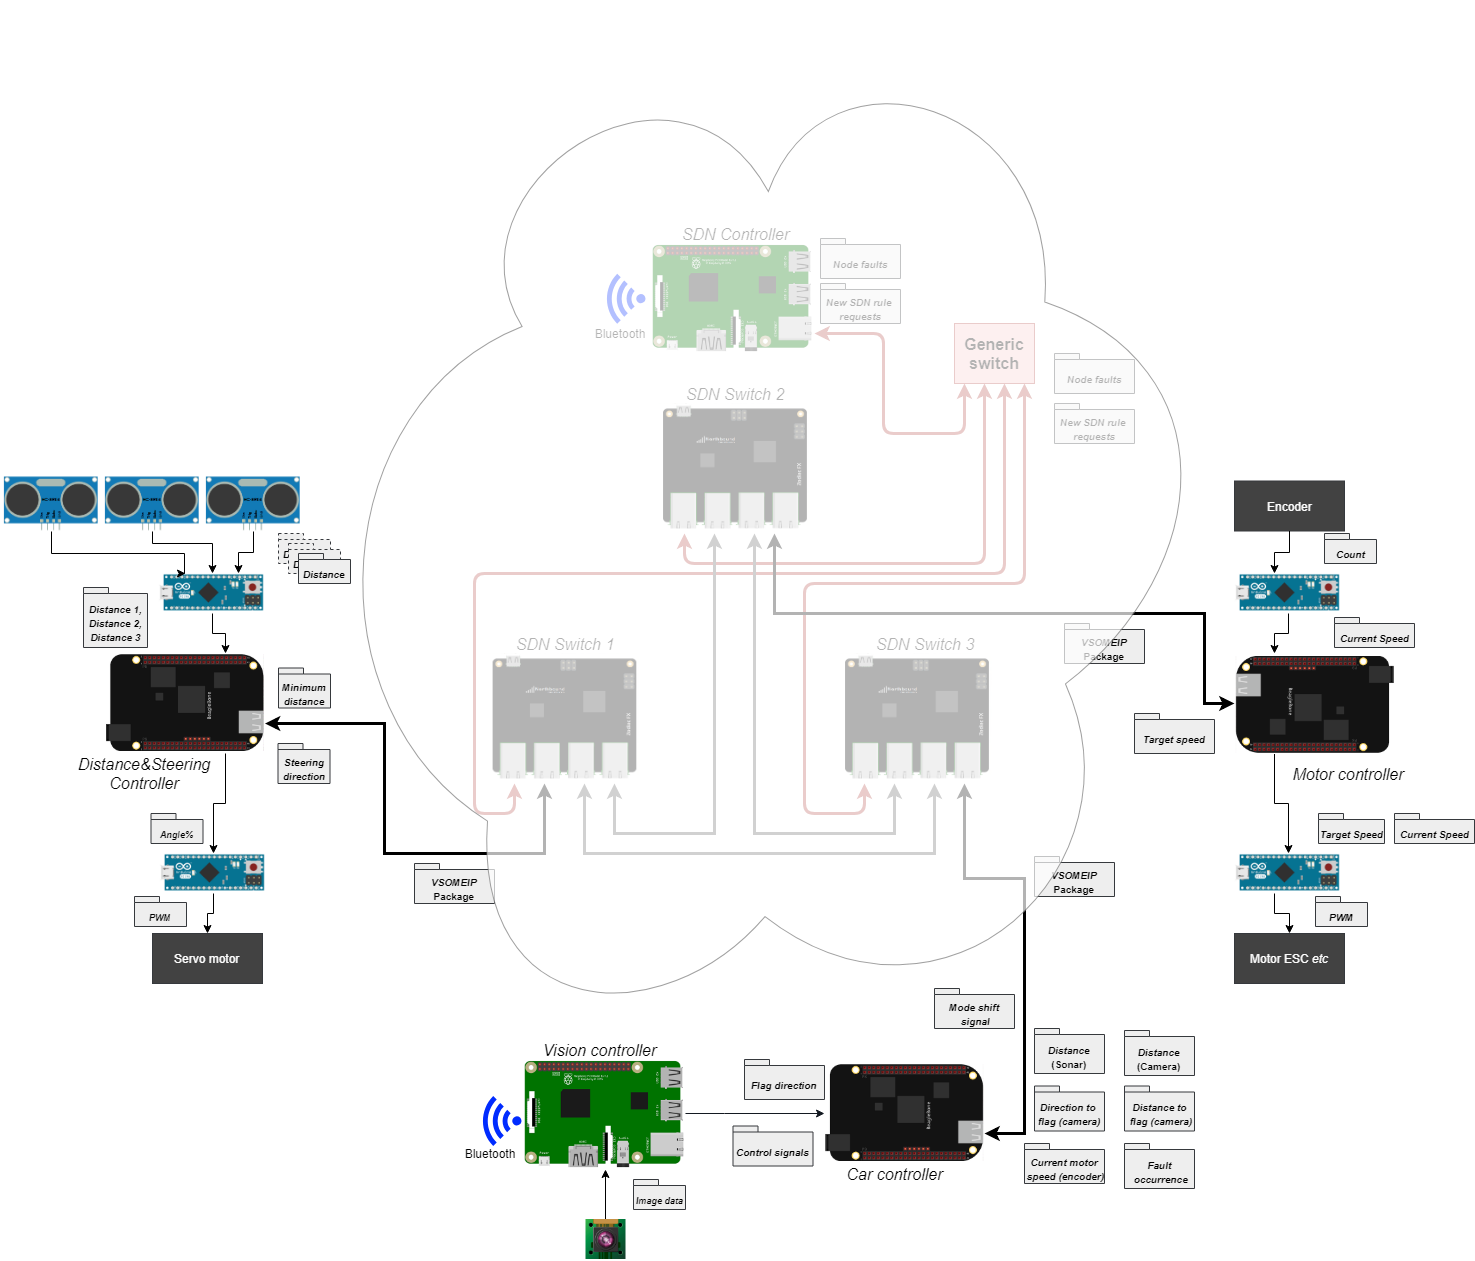
\includegraphics[width=1\linewidth]{network.png}
        \caption{Network topology}
        \label{pic:network}
        \end{figure}
    
\end{block}



%----------------------------------------------------------------------------------------
%	
%----------------------------------------------------------------------------------------



%----------------------------------------------------------------------------------------

\end{column} % End of the first column

\begin{column}{.03\textwidth}\end{column} % Empty spacer column
 
\begin{column}{.465\textwidth} % The second column

    %----------------------------------------------------------------------------------------
%	Control and Sensors 
%----------------------------------------------------------------------------------------

\begin{block}{Control and sensors}

    \begin{itemize}
        \item There are three ultrasonic distance sensors placed in front of the car to detect obstacles. The three sensors are placed so that they provide directional distance data, to enable fast avoidance if obstacles are detected on the left or right hand side of the cars heading. 
        
        \item By using a Raspberry Pi camera, the car should be able to detect traffic signs, but a simplification was made to only detect a set of colours. If there is a green sign in the field of view of the car, it will follow the sign. If the sign is red, the car will stop.  
        
        \item An IR sensor placed close to the left rear wheel to measure the speed. Aluminium tape is placed evenly spaced inside the wheel to reflect the light from the sensor so that it registers a pulse. By counting the pulses and measuring time one can extract speed information.
    \end{itemize}
    
    \end{block}



    \begin{block}{Assembly}

        \begin{itemize}
            \item The car was assembled with laser cut acrylic plastic, designed to secure the hardware on top of the frame. A test rig using the partially assembled car is shown in figure \ref{fig:car1}.
            \item The design of the assembly platform was done in Autodesk Fusion 360.
            
            
            \item The car is powered by a lipo battery with 2 cells. This is used to power the engine and all the components of the car via the PCB designs. One switch requires 9v to run so a boost converter is used to convert the otherwise required 5v supply.
              
        \end{itemize}
    
    \end{block}
%----------------------------------------------------------------------------------------
\begin{block}{Figure of the car}
    \begin{figure}
        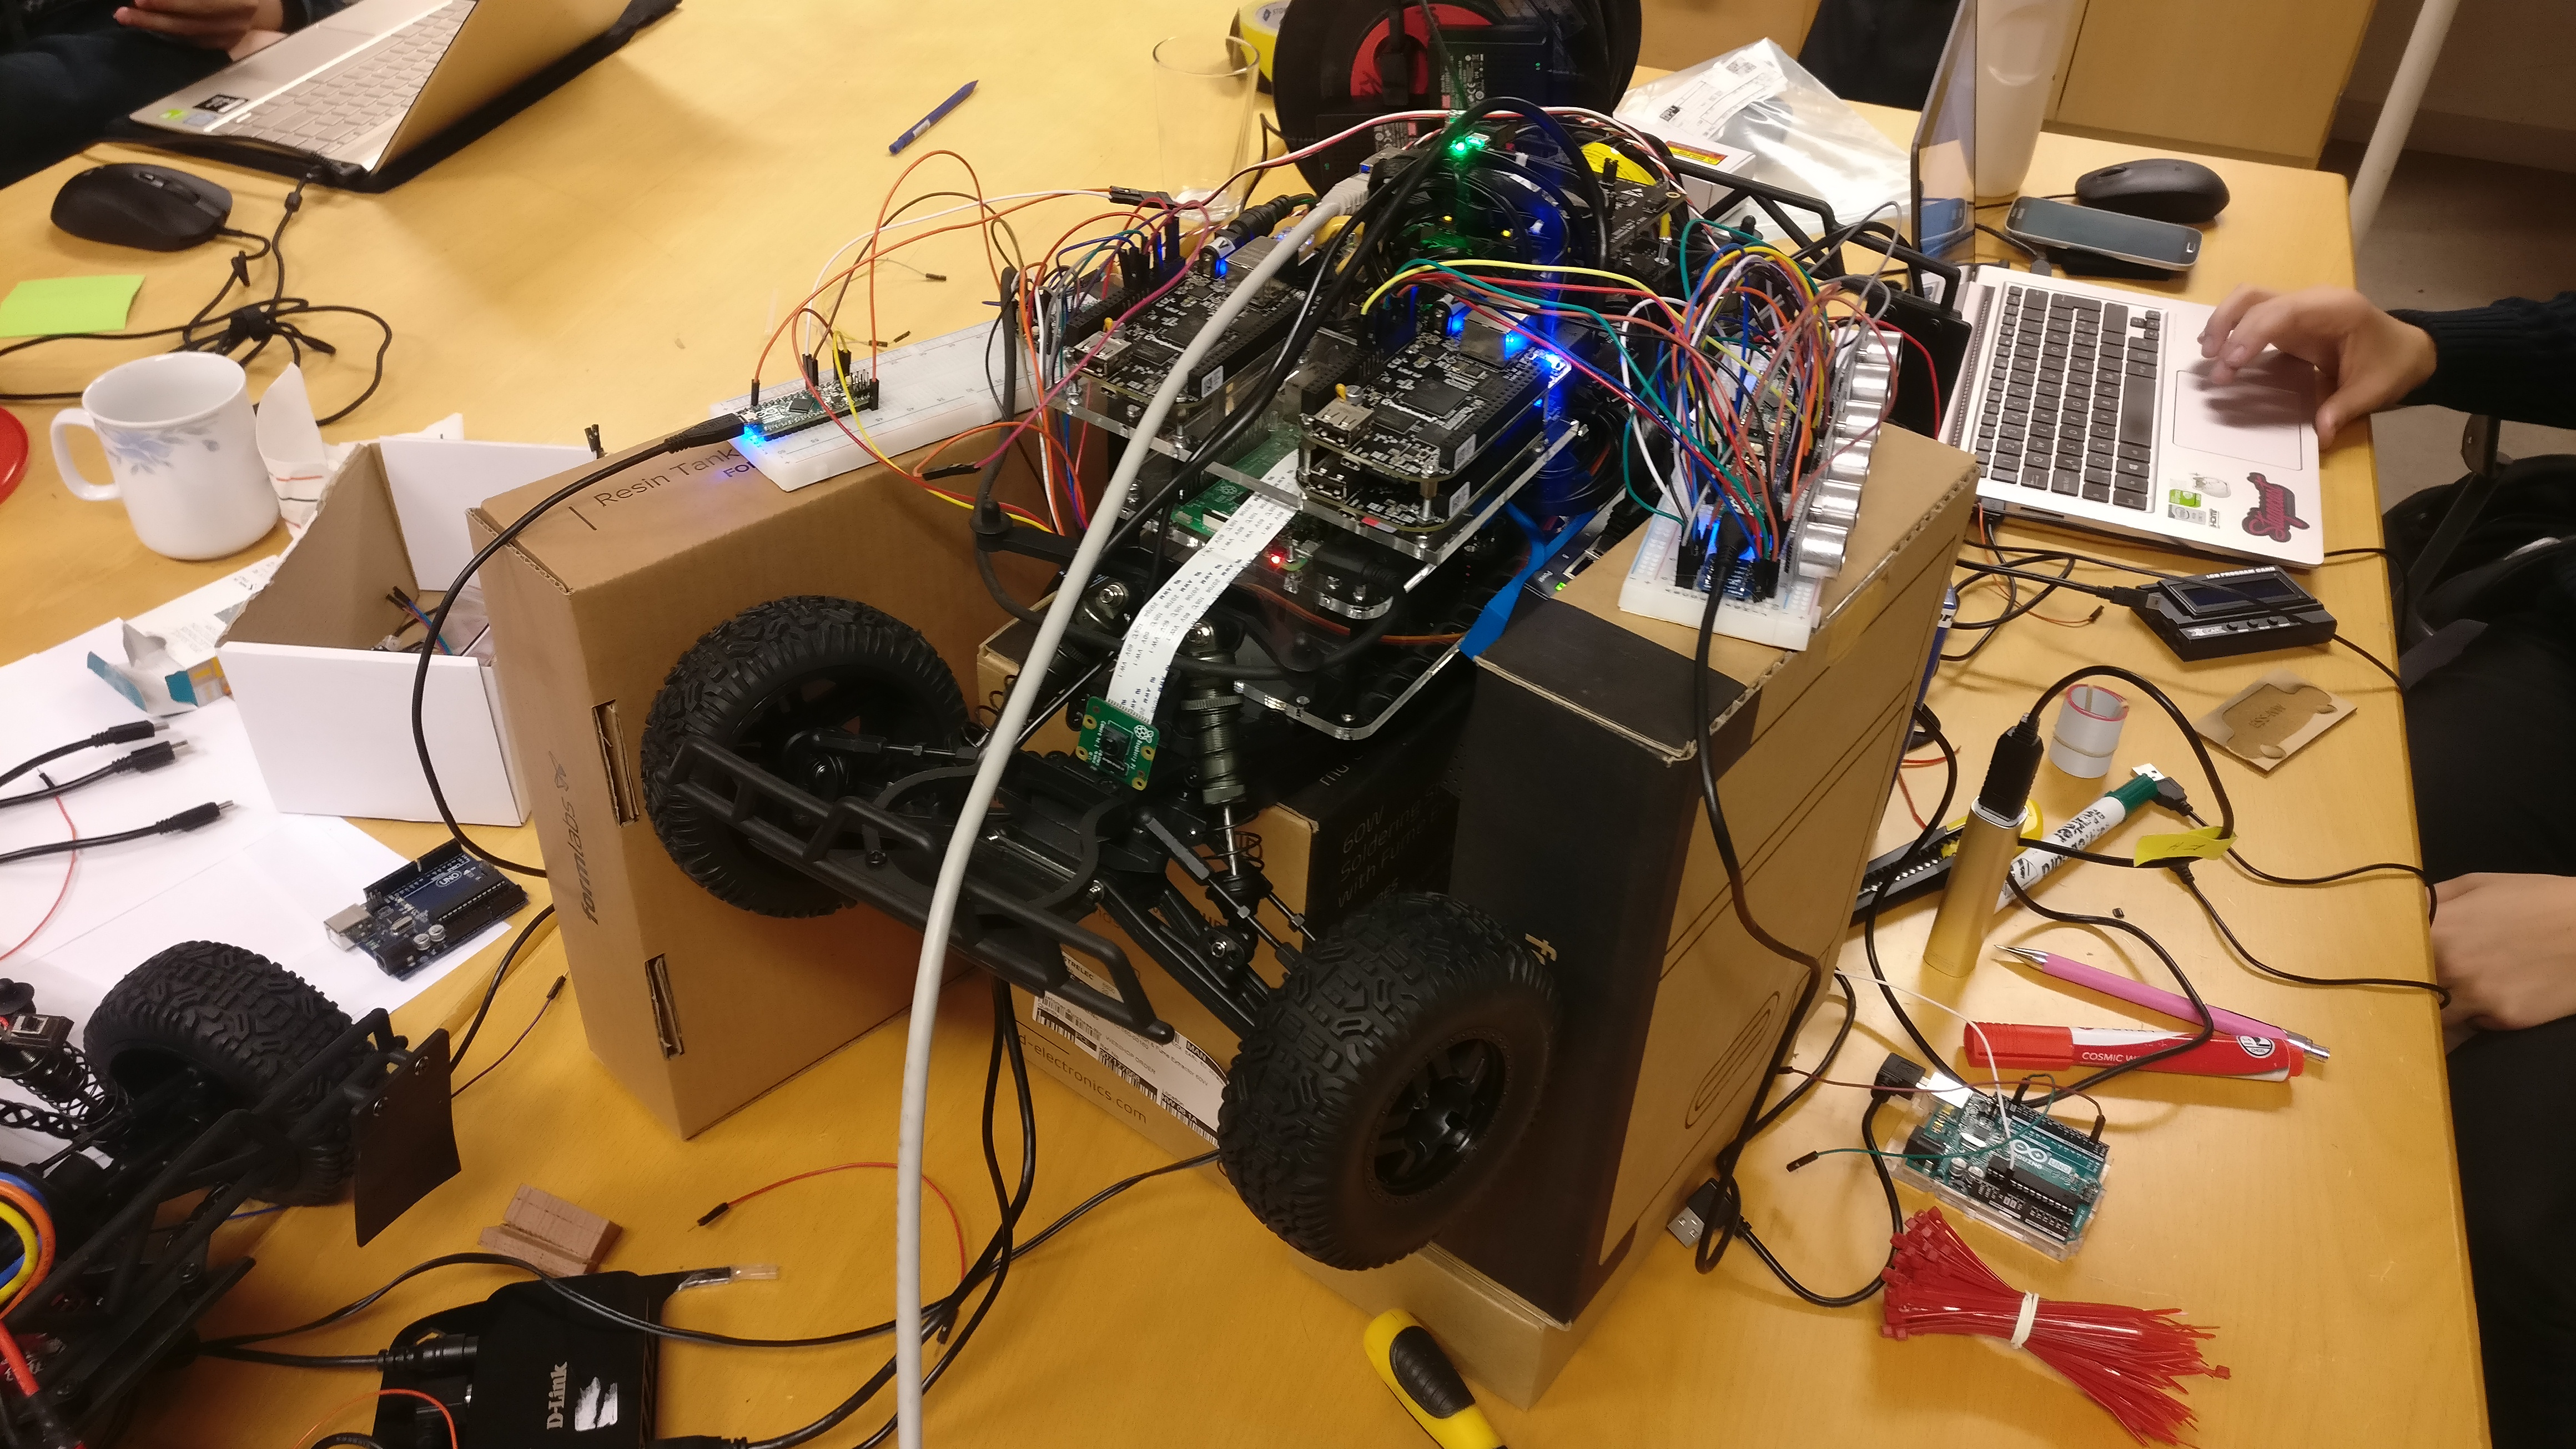
\includegraphics[width=1\linewidth]{car1.jpg}
        \label{fig:car1}
        \caption{Picture of the car}
    \end{figure}
\end{block}

%------------------------------------------------

%\begin{block}{Figure of the car}
%    \begin{figure}
%        \includegraphics[width=1\linewidth]{car2.jpg}
%        \label{gig:car2}
%        \caption{Picture of the car}
%    \end{figure}
%\end{block}
%
%


%----------------------------------------------------------------------------------------
%	ACKNOWLEDGEMENTS
%----------------------------------------------------------------------------------------

\begin{block}{Acknowledgments}

\begin{itemize}
\item We want to thank the project owners for their support they have given us throughout this project. 
\end{itemize}

\end{block}

%----------------------------------------------------------------------------------------
%	INFORMATION
%----------------------------------------------------------------------------------------

\setbeamercolor{block title}{fg=black,bg=orange!70} % Change the block title color

\begin{block}{Prodject Information}

\begin{itemize}
\item Github: \href{https://github.com/fhyy/MF2063-ESS-NW-CAR}{https://github.com/fhyy/MF2063-ESS-NW-CAR}

\end{itemize}

\end{block}

%----------------------------------------------------------------------------------------

\end{column} % End of the second column

\begin{column}{.015\textwidth}\end{column} % Empty spacer column

\end{columns} % End of all the columns in the poster

\end{frame} % End of the enclosing frame

\end{document}